
\chapter{Einschränkung der Kopplungsparameter durch Supernovae}

Im Folgenden betrachten wir einige der Argumente, die genutzt werden können, um die Kopplungsparameter zwischen Majoronen und Neutrinos einzuschränken, näher.
Konkret gehen wir auf die Einschränkungen durch Neutrinospektren, die es uns ermöglichen, die Kopplungsparameter $g_1$ und $g_2$ einzuschränken, und die Einschränkungen aus der Majoronenluminosität durch SN1987A ein,
die uns eine Obergrenze für $|\tilde{g}_{i j}|$ in Abhängigkeit der Majoronenmasse liefert.
Zusätzlich wird kurz das aktuelle Limit auf die Neutrinomasse $m_1$ diskutiert.

\section{Grenzen durch Neutrinospektren}
\label{subsec:spektrengrenzen}

Durch Majoronen induzierte Flavourübergänge der Neutrinos der Form $\tilde{\nu}^\pm_i \rightarrow \tilde{\nu}^\mp_j + J$ können das Energiespektrum der einzelnen Neutrinogenerationen merklich verschieben. 
Dabei muss beachtet werden, dass die Wirkungsquerschnitte der unterschiedlichen Neutrinos innerhalb einer typischen Supernova nicht übereinstimmen.
Diese Diskrepanz stammt daher, dass $\nu_\mu$ und $\nu_\tau$ nur über neutrale Ströme mit dem Supernovamedium interagieren können.
Innerhalb von Supernovae verhalten $\nu_\mu$ und $\nu_\tau$ sich nahezu gleich.
Elektronneutrinos $\nu_e$ können dagegen nicht nur über neutrale, sondern auch über geladene Ströme mit dem Medium wechselwirken.
So können sie unter Abstrahlung eines $W$-Bosons mit den im Überfluss vorhandenen Elektronen interagieren, während Wechselwirkungen von $\nu_\mu$ und $\nu_\tau$ mit der Materie in den dichteren Regionen des sterbenden Sterns kaum zustande kommen.
Es entsteht also ein Spektrum niedrigerer Temperaturen für $\nu_e$ und höherer Temperaturen für $\nu_\mu$ und $\nu_\tau$, dass durch Neutrinozerfälle verzerrt werden kann.
Berücksichtigen wir nun zusätzlich zur Zerfallswahrscheinlichkeit $N_\text{decay}$ außerdem die Oszillationswahrscheinlichkeit $N_\text{osc}$ der Neutrinos nach dem Verlassen seiner Energiesphäre mit Radius $R_{E, \tilde{\nu}^\pm_i}$, 
bis sie hier auf der Erde ankommen, lässt sich die effektive Wahrscheinlichkeit, dass ein Neutrino mit seinem ursprünglichen Flavour die Erde erreicht, als
\begin{equation}
    N = N_\text{decay} \cdot N_\text{osc}
    \label{eq:survivalprob}
\end{equation}
schreiben \cite{supernovaboundsdasandere}.

Die Zerfallswahrscheinlichkeit ist dabei gegeben durch
\begin{equation}
    N_\text{decay}(\tilde{\nu}^\pm) \cong \exp \left(- \int^\infty_{R_{E, \tilde{\nu}^\pm_i}} \mathrm{d}r \, \sum_j \Gamma(\tilde{\nu}^\pm_i \rightarrow \tilde{\nu}^\mp_j + J) \right) \,.
    \label{eq:zerfallswkeit}
\end{equation}
In relativistischer Näherung, die wir hier bereits zur Bestimmung der Materieeigenzustände verwendet haben, lässt sich die Zerfallsrate $\Gamma(\tilde{\nu}^\pm_i \rightarrow \tilde{\nu}^\mp_j + J)$ durch
\begin{equation}
    \Gamma(\tilde{\nu}^\pm_i \rightarrow \tilde{\nu}^\mp_j + J) = \frac{|\tilde{g}^2_{i j}|}{16 \pi} \left(V_i - V_f \right)
    \label{eq:zerfallsrate}
\end{equation}
ausdrücken, wobei $V_i - V_f$ die Potentialdifferenz zwischen Anfangs- und Endzustand beschreibt.

Die Oszillationswahrscheinlichkeit hängt stark von der gewählten Massendifferenz und dem Mischungswinkel zwischen den Neutrinos ab.
Wir fokussieren uns hier auf die LMA-MSW, also die Large-Mixing-Angle MSW-Lösung, die einen großen Mischungswinkel annimmt.
Wie in \cite{ueberlebenswkeit} genauer erläutert ergibt sich so eine Oszillationswahrscheinlichkeit von
\begin{equation}
    N_\text{osc} = 1 - \left[\sin^2\theta_\odot - \sin 2\theta_m \sin\left(2\theta_\odot - 2 \theta_m\right) \sin^2 \left(\frac{\pi d}{l_m}\right)\right] \,,
    \label{eq:osziwkeit}
\end{equation}
wobei
\begin{equation*}
    l_m = \frac{4 \pi E}{\Delta m^2_\odot} \frac{\sin2\theta_m}{\sin2\theta_\odot}
\end{equation*}
die Oszillationslänge und $\theta_m$ den Mischungswinkel der Neutrinos in Materie, die sie auf einer Distanz $d$ in der Erde bis zum Detektor durchdringen, beschreibt.
Wir gehen davon aus, dass es nur zu einer Mischung zwischen Elektron- und Myonneutrinos kommt, der Mischungswinkel $\theta_m$ lässt sich also mit $\theta_\odot$ identifizieren.
So lassen sich, wenn wir, wie in \cite{supernovaboundsdasandere} gezeigt, die entsprechenden, fehlenden Größen in \eqref{eq:osziwkeit} einsetzen, die Kopplungsparameter $g_1$ und $g_2$ auf einige $10^{-4}$ einschränken.
Wir werden später sehen, dass die so gefolgerten Grenzen auf $g_1$ für den Großteil unserer Betrachtung keine wirkliche Relevanz hat, uns aber erlaubt, die erstellten Plots unbesorgt auf $g_1 < 10^{-4}$ zu begrenzen. 

\section{Grenzen aus der Luminosität von SN1987A}

Die bekannteste und für die Astrophysik wichtigste Kernkollaps-Supernova ist die Supernova SN1987A.
Sie ist mit nur $157$ Lichtjahren Entfernung die erdnächste Supernova, die seit einigen Jahrhunderten beobachtet werden konnte und bietet mit ihrer großen Helligkeit die Möglichkeit, zum ersten Mal Supernovae näher zu untersuchen.
Mithilfe der Cherenkov-Detektoren Kamiokande II und Irvine-Michigan-Brookhaven gelang es, einige Events der SN1987A zu detektieren und so Grenzen auf die Luminosität emittierter Teilchen simulieren zu können.
Wie in \cite{neutrinolumi} gezeigt ergibt sich unter der Annahme, dass die Rate des Energieverlusts $\epsilon_a$ durch $\epsilon_a \lesssim 1 \cdot 10^{19} \,\text{erg} \,\text{g}^{-1} \,\si{\second}^{-1}$ beschränkt ist,
eine Neutrinoluminosität von
\begin{equation}
    L_\nu (1 \,\si{\second}) = \num{4.4} \cdot 10^{52} \,\text{erg} \si{\second}^{-1}
    \label{eq:neutrinolumi}
\end{equation}
eine Sekunde nach dem Kern-Rebound.
Dabei wurden Effekte der Rotverschiebung, durch die Neutrinos auf dem Weg von der Supernova bis zum Detektor Energie verlieren, berücksichtigt.
Mithilfe eines numerisch ermittelten Majoronenspektrums lässt sich die Luminosität dieser zu
\begin{equation}
    L_J (1 \,\si{\second}) = \num{6.46} \cdot 10^{68} \left(|g_{i j}| m_J \,\si{\mega\eV}^{-1} \right) \,\text{erg} \si{\second}^{-1}
\end{equation}
bestimmen, wobei $m_J$ die kinetische Energie der Majoronen beschreibt.
Als sinnvoller Majoronenenergiebereich kann $\SI{100}{\eV} \lesssim m_J \lesssim \SI{100}{\mega\eV}$ gefunden werden.
Da wir hier Zerfälle $J \rightarrow \nu \bar{\nu}$ annehmen, setzen wir voraus, dass die Majoronenluminosität nicht niedriger als die Neutrinoluminosität werden kann und erhalten so
\begin{equation*}
    |g_{i j}| m_J < \num{0.83} \cdot 10^{-8} \,\si{\mega\eV}
\end{equation*}
und damit eine Obergrenze von
\begin{equation}
    |g_{ij}| < \frac{\num{0.83} \cdot 10^{-8} \,\si{\mega\eV}}{m_J}
    \label{eq:gijlimit}
\end{equation}
auf die Kopplungsparameter $|g_{i j}|$.


\section{Neutrinomassengrenze aus KATRIN}
\label{subsec:KATRIN}

Das KATRIN-Experiment in Karlsruhe ist in der Lage, die Masse des Elektronneutrinos stark einzuschränken.
Dies ist möglich, indem das kontinuierliche Energiespektrum der Elektronen beim $\beta$-Zerfall genauestens untersucht wird, genauer genommen das Abknicken dieses Spektrums in der Nähe der maximalen Elektronenenergie.
Dieser Knick ist näher in \autoref{fig:elektronenspektrum} dargestellt.
\begin{figure}[H]
    \centering
    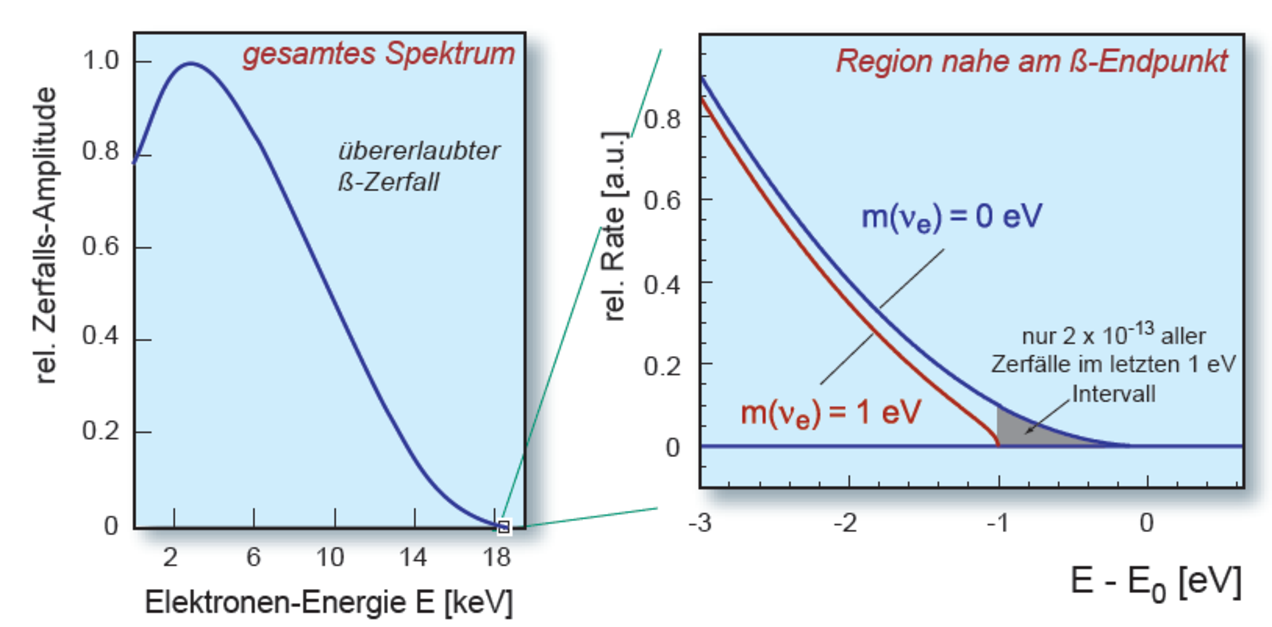
\includegraphics[width=.5\textwidth]{figures/Elektronenspektrum.pdf}
    \caption{Spektrum der Elektronen beim $\beta$-Zerfall. Die linke Kurve zeigt das gesamte Spektrum von der minimalen bis zur maximalen Energie, die das Elektron während des Zerfalls erhält. Rechts
            ist hochenergetische Ende der Kurve vergrößert dargestellt. Es wird ein Vergleich zwischen dem Kurvenverlauf unter der Annahme eines masselosen Neutrinos $m(\nu_e) = 0$ und dem Kurvenverlauf unter Freisetzung
            eines Elektronneutrinos mit einer Masse von $1 \si{\eV}$ hergestellt. Charakteristisch ist das Abknicken der Kurve für $m(\nu_e) \neq 0$. Dieses Abknicken stammt daher, dass das Elektron nicht länger
            die maximale Stoßenergie besitzen kann, sobald das Neutrino Masse besitzt \cite{elektronenspektrum}.}
    \label{fig:elektronenspektrum}
\end{figure}
Durch die Analyse der Position dieses Knicks konnte die Neutrinomasse Anfang $2022$ auf $m_1 < \SI{0.8}{\eV}$ \cite{KATRINneutrinogrenze} eingeschränkt werden.
Gemeinsam mit den in \autoref{subsec:spektrengrenzen} gefundenen Einschränkungen auf $g_1$ und damit auch auf $g_2$ lässt sich so das Fenster wählen, in dem die erstellten Plots relevant sind.



\section{Ausschlussregionen der Kopplungsparameter}
\label{sec:kopplungen}

Mit den bisher zusammengestellten Einschränkungen auf $g_1$, $m_1$ und $|g_{i j}|$ ist es uns möglich, Grafiken zu erstellen, die uns die zulässigen Bereiche für $g_1$ und $m_1$ deutlich machen.
Dazu betrachten wir die einzelnen Einträge in \eqref{eq:materiekoppmat} und nutzen die Ausdrücke in \eqref{eq:g2g3}, um $|g_{i j}|$ nur in Abhängigkeit von $g_1$ und $m_1$ zu schreiben.
Somit ist es uns möglich, anschließend wahlweise $g_1$ in Abhängigkeit von $m_1$ oder $m_1$ in Abhängigkeit von $g_1$ auszudrücken.
Hier entscheiden wir uns für $g_1 (m_1)$, da ein analytisches Umstellen unter Berücksichtigung von $\theta_{1 3} \neq 0$ nicht mehr möglich ist.
Für alle folgenden Plots werden die LMA-MSW-Werte
\begin{align}
    \sin^2\theta_\odot &= \num{0.307}\,, && \sin^2\theta_{13} &= \num{0.020}\,, \\ \Delta m^2_\odot &= \num{7.53} \cdot 10^{-5} \si{eV}^2\,, && \Delta m^2_\text{atm} &= \num{2.453} \cdot 10^{-3} \si{\eV}^2
    \label{eq:LMAMSW}
\end{align}
und die maximal als sinnvoll erachtete Majoronenmasse von 
\begin{equation*}
    m_J = \SI{100}{\mega\eV}
\end{equation*}
\cite{neutrinospdg, newlimit} verwendet, die nach \eqref{eq:gijlimit} einer oberen Grenze von
\begin{equation*}
    |g_{ij}| < \num{0.83} \cdot 10^{-6}
\end{equation*}
entspricht.

Beginnen wir zunächst mit der Kopplung $g_{ee}$.
Hier gehen wir die Rechnung einmal Schritt für Schritt durch, da die Rechenschritte allerdings nur aus Umformungen und trivialen Operationen besteht und für alle Kopplungen dem gleichen Schema folgen, werden wir auf die Berechnungen der anderen
Kopplungen nicht näher eingehen.

Im Folgenden nutzen wir die platzsparende Notation $c_{ij} = \cos{\theta_{ij}}$ und $s_{ij} = \sin{\theta_{ij}}$.
Rechnen wir \eqref{eq:materiekoppmat} konkret aus, gilt
\begin{equation}
    g_{ee} = c^2_{1 2} c^2_{1 3} g_1 + s^2_{12} c^2_{13} \mathrm{e}^{-2 i \delta_1} g_2 + s^2_{13} \mathrm{e}^{-2 i \delta_2}  g_3 \,.
    \label{eq:g_ee}
\end{equation}
Unter der Nutzung von
\begin{equation*}
    g_2 = g_1 \sqrt{1 + \frac{\Delta m^2_\odot}{m^2_1}}
\end{equation*}
aus \eqref{eq:g2g3} erhalten wir
\begin{equation*}
    g_{ee} = g_1 \left(c^2_{1 2} c^2_{1 3} + \sqrt{1 + \frac{\Delta m^2_\odot}{m^2_1}}s^2_{12} c^2_{13} \mathrm{e}^{-2 i \delta_1} + \sqrt{1 + \frac{\Delta m^2_\odot + \Delta m^2_\text{atm}}{m^2_1}} s^2_{13} \mathrm{e}^{-2 i \delta_2}\right)
\end{equation*}
Dividieren wir durch den ausgeklammerten Ausdruck auf der rechten Seite, erhalten wir
\begin{equation}
    g_1(m_1,g_{ee}) = \frac{g_{ee}}{\left(c^2_{1 2} c^2_{1 3} + \sqrt{1 + \frac{\Delta m^2_\odot}{m^2_1}}s^2_{12} c^2_{13} \mathrm{e}^{-2 i \delta_1} + \sqrt{1 + \frac{\Delta m^2_\odot + \Delta m^2_\text{atm}}{m^2_1}} s^2_{13} \mathrm{e}^{-2 i \delta_2}\right)} \,.
    \label{eq:g_1g_ee}
\end{equation}

Da die CP-verletzenden Phase $\delta_1,\delta_2$ frei wählbar sind, wählen wir hier zur Darstellung der Kopplung stets die beiden Extreme $\delta_i = 0$, also einen maximal positiven, und $\delta_i = \frac{\pi}{2}$, also einen maximal negativen Phasenbeitrag.
Je nach Kombination der beiden Phasen können sich die Nennerterme, zumindest teilweise, gegenseitig annullieren.
So entstehen unterschiedliche Zweige, wie sie in \autoref{fig:g_eefinal} zu erkennen sind.
Dazu sei gesagt, dass, da sich die Obergrenze nur auf den Betrag von $g_{i j}$ bezieht, unterschiedliche Kurven für $g_{ij} = \pm \frac{\num{0.83} \cdot 10^{-8}}{m_J}$ entstehen.
Zusätzlich sind die $x$- und $y$-Achsen aller folgenden Plots getauscht, um eine bessere Vergleichbarkeit mit \cite{päspaper} zu erreichen.
\begin{figure}[H]
    \centering
    \includegraphics[width=0.8\textwidth]{build/g_eefinal.pdf}
    \caption{Kopplungsparameter $g_1(m_1,g_{ee})$ in Abhängigkeit von $m_1$ für eine Majoronenmasse von $m_J = \SI{100}{\mega\eV}$. Die rote Fläche kennzeichnet dabei den durch KATRIN ausgeschlossen Massenbereich von $m_1 > \SI{0.8}{\eV}$.
    Durchgezogene Linien bezeichnen dabei Kurven mit positiver, gestrichene Linien immer Kurven mit negativer Obergrenze.}
    \label{fig:g_eefinal}
\end{figure}
Auffällig ist, dass für die Wahl einer negativen Obergrenze die Äste mit $\delta_1 = \delta_2 = 0$ sowie $\delta_1 = 0$ und $\delta_2 = \frac{\pi}{2}$ im gewählten Bereich nicht existieren.
Dies stammt daher, dass sich die Phasenfaktoren in \eqref{eq:g_1g_ee} so weit kompensieren, dass der Gesamtausdruck für $g_1$ negativ wird.
Da wir hier allerdings nur Kopplungen $g_1 > 0$ betrachten, treten diese Kurven nicht auf.
Selbiges gilt auch für scheinbar nicht existierende Kurven in allen weiteren Plots.

Die Ausschlussregion unserer Parameter wählen wir immer möglichst konservativ, sprich so, dass die zugelassene Region so wenig wie möglich, aber so viel wie nötig eingeschränkt wird.
Das erreichen wir hier, indem wir den positiven und negativen Zweig mit $\delta_1 = \frac{\pi}{2}, \delta_2 = 0$ kombinieren.
Ausgeschlossen werden nun alle Wertepaare, die unterhalb der gestrichenen und oberhalb der durchgezogen roten Kurve liegen.
Wird $m_1$ groß gegen die Massendifferenzen $\Delta m^2_\text{atm}$ bzw. $\Delta m^2_\odot$,   
Auffällig ist auch das asymptotische Verhalten der Äste für verhältnismäßig große $g_1$.
Wird $g_1$ groß gegen die gewählte Grenze von $g_{ee}$, gilt näherungsweise $g_1 \approx \text{const}$.
Dieses Verhalten lässt sich in den nach oben divergierenden Zweigen der positiven Obergrenzen erkennen.
Ähnlich existiert ein Resonanzwert $m_{1,0}$ bei dem $g_1$ aufgrund der Phaseninteraktionen im Nenner erst divergiert und bei Erreichen von $m_{1,0}$ einbricht.

Analog gehen wir für die restlichen Kopplungen vor.
So ergibt sich aus
\begin{equation*}
    g_{e \mu'} = -s_{12}c_{12}c_{13} g_1 + c_{12} s_{12} c_{13} \mathrm{e}^{-2 i \delta_1} g_2
\end{equation*}
für die Kopplung $g_{e \mu'}$
\begin{equation}
    g_1(m_1,g_{e \mu'}) = \frac{2 g_{e \mu'}}{\sin(2\theta_\odot) \cos\theta_{13} \left(\sqrt{1 + \frac{\Delta m^2_\odot}{m^2_1}} \mathrm{e}^{-2 i \delta_1} - 1\right)} \,,
    \label{eq:g_1g_emu}
\end{equation}
für $g_{\mu' \mu'}$ folgt aus
\begin{equation*}
    g_{\mu' \mu'} = s^2_{12} g_1 + c^2_{12} \mathrm{e}^{-2 i \delta_1} g_2
\end{equation*}
\begin{equation}
    g_1(m_1, g_{\mu'\mu'}) = \frac{g_{\mu'\mu'}}{s^2_{1 2} + \sqrt{1 + \frac{\Delta m^2_\odot}{m^2_1}} c^2_{12} \mathrm{e}^{-2 i \delta_1}} \,.
    \label{eq:g_1g_mumu}
\end{equation}
und für $g_{\tau' \tau'}$ aus
\begin{equation*}
    g_{\tau' \tau'} = c^2_{21} s^2_{13} g_1 + s^2_{12}s^2_{13} \mathrm{e}^{-2 i \delta_1} g_2 + c^2_{13} \mathrm{e}^{-2 i \delta_2} g_3
\end{equation*}
\begin{equation}
    g_1(m_1,g_{\tau'\tau'}) = \frac{g_{\tau'\tau'}}{c^2_{12}s^2_{13} + \sqrt{1 + \frac{\Delta m^2_\odot}{m^2_1}} s^2_{12} s^2_{13} \mathrm{e}^{-2 i \delta_1} + \sqrt{1 + \frac{\Delta m^2_\odot + \Delta m^2_\text{atm}}{m_1}}c^2_{13} \mathrm{e}^{-2 i \delta_2}}\,.
    \label{eq:g_1g_tautau}
\end{equation}
Auf den ersten Blick ähnelt \eqref{eq:g_1g_tautau} sehr stark \eqref{eq:g_1g_ee} mit dem einzigen Unterschied, dass $s^2_{13}$ und $c^2_{13}$ vertauscht sind.
Jedoch sind hier die Beiträge von $s^2_{13}$ so klein, dass die Kurven $g_1(m_1,g_{\tau'\tau'})$ unterschiedlicher Phasen nahezu übereinstimmen und es nicht zu dem bei $g_1(m_1, g_{ee})$ beobachteten Verhalten kommt.
Das Verhalten von $g_1(m_1, g_{\tau'\tau'})$ wird im Grunde nur vom letzten Nennerterm beeinflusst.

Wählen wir für jeden Parameter $g_{ij}$ einzeln die konservativste Ausschlussregion und fassen alle übrigen Kurven in einer einer Grafik zusammen, ergibt sich \autoref{fig:g_ijfinal}.
\begin{figure}[H]
    \centering
    \includegraphics[width=.8\textwidth]{build/g_ijfinal.pdf}
    \caption{Kopplungsparameter $g_1$ in Abhängigkeit von $m_1$. Übrig bleiben die bereits erwähnte Ausschlussregion aus $g_{ee}$ mit $\delta_1=\frac{\pi}{2}, \delta_2=0$ in blau, 
    die positive Obergrenze mit $\delta_1 = 0$ aus $g_{e \mu}$ in grün, die negative Obergrenze mit $\delta_1 = \frac{\pi}{2}$ aus $g_{\mu\mu}$ in violett und die negative Obergrenze mit $\delta_1 = 0, \delta_2 = \frac{\pi}{2}$ aus $g_{\tau'\tau'}$ in rot.
    Die leicht durchscheinende rote Fläche kennzeichnet erneut den ausgeschlossenen Neutrinomassenbereich $m_1 > \SI{0.8}{\eV}$.}
    \label{fig:g_ijfinal}
\end{figure}

Um die finale Ausschlussregion zu erhalten, bleibt uns nun keine andere Wahl, als $g_1(m_1,g_{\tau'\tau'})$ als Grenze zu wählen, sodass sich die in \autoref{fig:exclusionregionfinal} eingefärbte, simple Fläche ergibt.

\begin{figure}[H]
    \centering
    \includegraphics[width=.8\textwidth]{build/exclusionregionfinal.pdf}
    \caption{Finale Ausschlussregion der Parameter $g_1$ und $m_1$, nur noch gegeben durch die Kurve $g_1(m_1, g_{\tau'\tau'})$. Alle Wertepaare, die innerhalb der roten oder violett gefärbten Flächen liegen, werden ausgeschlossen.}
    \label{fig:exclusionregionfinal}
\end{figure}


